%%%%%%%%%%%%%%%%%%%%%%%%%%%%%%%%%%%%%%%%%%%%%%%%%%%%%%%%%%%%%%%%%%%%%%%%%%%%%%%%
%% PRISM — Artificial Intelligence and Law (Springer) submission
%% Springer Nature LaTeX template (sn-jnl.cls).
%%
%% BEFORE COMPILING: this file requires Springer's sn-jnl.cls and the sn-apa
%% bibliography style. The easiest path is Overleaf → "New Project" →
%% "Springer Nature Article" template, then replace its main .tex with this
%% file and its .bib with sn-article.bib. See paper/NOTES_before_submission.md.
%%
%% Reference style: sn-apa (author–year), which is the style used by
%% Artificial Intelligence and Law. To switch to numbered, change the class
%% option to sn-mathphys-num (one word) — see NOTES.
%%%%%%%%%%%%%%%%%%%%%%%%%%%%%%%%%%%%%%%%%%%%%%%%%%%%%%%%%%%%%%%%%%%%%%%%%%%%%%%%
\documentclass[sn-apa]{sn-jnl}

%% Packages already loaded by sn-jnl: graphicx, amsmath, amssymb, booktabs, etc.
\usepackage{graphicx}
\usepackage{multirow}
\usepackage{amsmath,amssymb}
\usepackage{booktabs}
\usepackage{algorithm}
\usepackage{algorithmicx}
\usepackage{algpseudocode}
\usepackage{url}
\usepackage[capitalise]{cleveref}

\raggedbottom

%% Portable rupee symbol (avoids depending on a font package; renders as "Rs.").
\providecommand{\rupee}{Rs.\,}

\begin{document}

\title[PRISM: Explainable Legal Policy Intelligence]{PRISM: From Clause to Consequence---An Explainable, Provenance-Linked Framework Bridging Legal Text Understanding and Agent-Based Socioeconomic Simulation}

\author*[1]{\fnm{[First]} \sur{[Last]}}\email{[corresponding.author]@karunya.edu.in}
\author[1]{\fnm{[Co-author]} \sur{[Last]}}\email{[coauthor]@karunya.edu.in}
\author[1]{\fnm{[Supervisor]} \sur{[Last]}}\email{[supervisor]@karunya.edu.in}

\affil*[1]{\orgdiv{Department of Computer Science and Engineering}, \orgname{Karunya Institute of Technology and Sciences}, \orgaddress{\city{Coimbatore}, \state{Tamil Nadu}, \country{India}}}

\abstract{Legal statutes encode conditional obligations, penalties, and
thresholds whose aggregate effect on a population is rarely evident from the
text, yet the two disciplines that could reveal it---legal natural language
processing (NLP) and agent-based policy modelling---remain disconnected. Legal
NLP systems stop at classification or summarisation; agent-based models begin
from hand-coded rules that domain experts spend months extracting by reading
legislation. We present PRISM, an end-to-end, local-first framework that closes
this gap. PRISM parses a statute, extracts structured causal rules with a
quantised local large language model (LLM) explained token-by-token by LIME and
transformer attention, translates those rules into the parameters of a
Mesa agent-based simulation of five income strata, and answers grounded,
source-cited questions over a multi-statute corpus using
retrieval-augmented generation. Its defining feature is \emph{full-chain
provenance}: every simulation outcome is mechanically traceable to the causal
rule, the source clause (page and bounding box), and the token-level
explanation that produced it---turning a black-box pipeline into an auditable
one. On a corpus of five Indian statutes we obtain retrieval recall@1/@8 of
$0.66$/$0.94$; a legal fine-tuned adapter (PRISM-Legal, QLoRA) improves causal
extraction $F_1$ over zero-shot; and per-type income calibration reduces
simulation sampler divergence $3.4\times$ versus an uncalibrated baseline
($\mathrm{KL}=0.068$ vs.\ $0.234$). The entire system runs on a consumer GPU
(4\,GB VRAM), demonstrating that transparent, auditable policy AI need not
depend on cloud infrastructure. We discuss the framework's implications for
legislative impact assessment and its limitations for quantitative policy
claims.}

\keywords{Legal NLP, Explainable AI, Agent-based modelling, Retrieval-augmented
generation, Policy analysis, Provenance, Large language models}

\maketitle

%%==========================================================================
\section{Introduction}\label{sec:intro}

Legislation is written to be applied, not merely read. A single statutory
clause may impose a duty, attach a penalty, and set a monetary threshold whose
combined effect falls unevenly across a population---raising revenue from some
groups, pushing others into non-compliance, and shifting the overall
distribution of burden. Understanding that effect is central to the practice of
law and policy, yet it is precisely what current computational tools leave
unaddressed. Two mature but disconnected research communities each solve one
half of the problem. Legal NLP has produced strong models for clause
classification, entity recognition, summarisation, and judgment prediction
\citep{chalkidis2020legalbert,chalkidis2022lexglue,bommarito2021lexnlp}; these
systems condense or label text but never ask what happens to real people when a
provision is enforced. Computational social science, meanwhile, uses
agent-based models (ABMs) to simulate how populations respond to policy
\citep{bonabeau2002abm,epstein1996growing,kazil2020mesa}; but these models
begin from rules that a domain expert has hand-coded after weeks of reading the
statute. \emph{No system connects legal-text understanding directly to
society-level impact simulation with an explainability layer at every stage.}

A concrete example fixes intuition. Consider a common statutory construct: a flat
late-filing fee of a fixed rupee amount, payable by any assessee who files after a
deadline. Read in isolation the clause is unremarkable. But a fixed fee is a
larger share of a small income than a large one, so its \emph{incidence} is
regressive---it falls hardest on those least able to pay, and, if enforcement is
credible, pushes low-income filers toward non-compliance while leaving wealthier
filers unaffected. Seeing this requires connecting three things a human expert
would otherwise assemble by hand: the clause's causal structure (late filing
$\rightarrow$ fixed fee), a model of how different income groups respond, and a
way to attribute the resulting distributional finding back to the originating
words. PRISM automates exactly this chain, and we return to this example as a
worked provenance case study in \cref{sec:casestudy}.

This disconnection has a second, subtler cost: opacity. Even where an
end-to-end pipeline could be assembled from existing components, the result
would be a black box in which a predicted societal outcome cannot be traced
back to the specific clause and model reasoning that produced it. For a
technology intended to inform legislative debate, the inability to answer
``\emph{which clause caused this, and why did the model read it that way?}'' is
disqualifying. Explainable AI (XAI) methods such as LIME
\citep{ribeiro2016lime} and SHAP \citep{lundberg2017shap} explain a single
model's prediction, but a statute-to-simulation pipeline chains many models;
explaining one link does not make the outcome auditable.

We address both problems with PRISM (Policy Rule Interpretation and
Socioeconomic Impact Modelling). PRISM is an integrated, local-first framework
that reads an Indian statute PDF and produces (i) structured causal rules, each
explained at the token level; (ii) an agent-based simulation of the statute's
socioeconomic incidence across five income strata; and (iii) a grounded,
source-cited question-answering interface over a multi-statute corpus. Binding
these together is a provenance spine: every simulation finding resolves,
mechanically and without recomputation, to the rule, the source clause with its
page and bounding box, and the token-level explanation behind it. The central
research question is:

\begin{quote}
\emph{Can an explainable AI system autonomously extract causal policy rules from
legal text and translate them into agent-based socioeconomic simulations that
predict differential impacts across population subgroups, with traceable
provenance from every simulation outcome back to its source legal clause---and
can it do so on commodity hardware?}
\end{quote}

\paragraph{Contributions.} This paper makes five contributions, each
substantiated in \cref{sec:arch,sec:results}:
\begin{enumerate}
  \item \textbf{An end-to-end statute-to-simulation pipeline} that requires no
  manual rule coding, connecting legal NLP to agent-based modelling
  (\cref{sec:arch}).
  \item \textbf{Full-chain, system-level provenance}: every simulation outcome
  is traceable to the causal rule, source clause (page/bounding box), and
  token-level XAI explanation. To our knowledge no prior legal-AI system
  provides this (\cref{sec:provenance}).
  \item \textbf{Automated ABM parameterisation from text} via a 16-template
  semantic matcher with an LLM fallback, converting legal rules into simulation
  parameters (\cref{sec:translator}).
  \item \textbf{A defensible incidence model} whose regressivity verdict is
  derived from effective tax rate across income strata---the textbook
  definition of incidence---rather than a fragile Gini trajectory
  (\cref{sec:simulation}), together with adaptive (Q-learning) compliance
  agents.
  \item \textbf{Consumer-GPU feasibility}: the complete pipeline---quantised LLM
  extraction, dual XAI, simulation, and retrieval-augmented
  generation---runs within 4\,GB of VRAM, showing that auditable
  interdisciplinary policy AI can be democratised (\cref{sec:setup}).
\end{enumerate}

We evaluate PRISM on a corpus of five Indian statutes anchored by the Income Tax
Bill, 2025, using both an out-of-domain public benchmark (LEDGAR) and
human-reviewed in-domain gold sets, and report retrieval, extraction,
explanation-fidelity, and simulation-validity results in \cref{sec:results}. We
are explicit throughout about what PRISM validates and what it does not: the
simulation is a defensible \emph{illustrative} incidence model, not a fitted
microsimulation, and we state this limitation plainly (\cref{sec:discussion}).

%%==========================================================================
\section{Related Work}\label{sec:related}

\subsection{Legal NLP}
Transformer models pre-trained on legal corpora, notably LEGAL-BERT
\citep{chalkidis2020legalbert}, established strong baselines for legal text
classification and were consolidated into the LexGLUE benchmark suite
\citep{chalkidis2022lexglue}. Task-specific resources such as CUAD
\citep{hendrycks2021cuad} for contract review and LEDGAR
\citep{tuggener2020ledgar} for provision classification supply labelled clauses,
and rule/ML hybrids such as LexNLP \citep{bommarito2021lexnlp} extract entities
and facts. These systems classify, tag, or summarise; none extract structured
\emph{causal} rules (condition--action--consequence triples) or connect their
output to a downstream simulation of societal effect. PRISM builds on this
tradition for its entity layer but treats extraction as the input to impact
modelling rather than the end product.

\subsection{Agent-based policy modelling}
Agent-based modelling is a well-established method for studying emergent
socioeconomic dynamics \citep{bonabeau2002abm,epstein1996growing}, with mature
toolkits---Mesa \citep{kazil2020mesa} among them---and a long history of tax and
welfare studies. The persistent bottleneck is parameterisation: rules and
behavioural parameters are specified by hand after expert reading of the source
policy. PRISM automates this step, generating simulation parameters directly
from extracted legal rules, and thereby positions itself as a bridge between
legal NLP and the ABM literature rather than a new simulation engine.

\subsection{Explainable AI}
Local surrogate methods (LIME, \citealp{ribeiro2016lime}) and additive
attribution (SHAP, \citealp{lundberg2017shap}) explain individual predictions,
and attention weights \citep{vaswani2017attention} offer a complementary,
model-internal view; surveys catalogue the breadth of such methods
\citep{guidotti2018survey}. All operate at the level of a single model. PRISM's
contribution is orthogonal: it chains explanations across modules so that a
\emph{system-level} outcome---a simulated distributional effect---inherits a
provenance trail down to source tokens.

\subsection{Retrieval-augmented generation and efficient LLMs}
Retrieval-augmented generation (RAG) grounds LLM output in retrieved evidence to
curb hallucination \citep{lewis2020rag,gao2023ragsurvey}, a property essential
in a legal setting where every claim must be attributable. Parameter-efficient
fine-tuning (LoRA, \citealp{hu2022lora}) and its quantised variant QLoRA
\citep{dettmers2023qlora}, together with compact instruction-tuned models such
as Phi-3.5-mini \citep{abdin2024phi3} and sentence encoders like Sentence-BERT
\citep{reimers2019sbert}, make it feasible to run this entire stack locally.
PRISM composes these advances under a strict 4\,GB VRAM budget.

\subsection{Legal impact assessment and regulatory analysis}
The practice PRISM ultimately serves---regulatory impact assessment---is
long-established in public administration: before enactment, an analyst estimates
who a proposed measure will affect and by how much. This work is overwhelmingly
manual, relying on expert reading of draft text and bespoke economic models, and
is therefore slow, costly, and difficult to reproduce or contest. Microsimulation
models used by finance ministries provide precise distributional estimates but
require unit-level administrative data and months of expert construction; ABMs
trade that precision for the ability to model behavioural response and emergent
compliance dynamics, but still demand hand-coded rules. PRISM occupies a
deliberately different point in this space: it is not a replacement for a fitted
microsimulation, but a rapid, transparent, first-pass screening tool that reads
the statute itself and produces a directional incidence assessment with a
complete audit trail---something no manual process delivers at the speed of a
single document upload.

\subsection{Causal information extraction from legal text}
Extracting condition--action--consequence structure is harder than entity tagging
because the relevant spans are often discontinuous and the causal link is
implicit in legal drafting conventions (``where\ldots, the assessee shall\ldots,
failing which\ldots''). Prior work has largely treated this as clause
classification or rhetorical-role labelling rather than structured triple
extraction. PRISM's use of a generative LLM to emit a typed causal rule, combined
with a rule-based cross-check and a span-similarity metric, is a pragmatic
response to the scarcity of gold causal annotations in statutory (as opposed to
contract) text.

\subsection{Faithfulness of explanations}
A recurring critique of post-hoc explanation is that a plausible-looking saliency
map need not reflect the model's actual computation. In a legal setting this is
not a philosophical nicety: an unfaithful explanation that a practitioner trusts
is actively harmful. We therefore treat explanation fidelity as a first-class,
reported quantity (the LIME local-surrogate $R^2$) rather than presenting
attributions as self-evidently trustworthy, and we complement the surrogate view
with a model-internal attention view so that the two can be compared.

\subsection{Positioning}
The novelty of PRISM is integrative. Individually, legal extraction, ABM,
LIME, and RAG are established. What does not exist in the literature is a single
pipeline that (a) extracts causal rules from primary legal text, (b) simulates
their population-level incidence, (c) answers grounded questions over the
corpus, and (d) makes every simulated outcome auditable back to a source clause
and its token-level explanation. \Cref{tab:positioning} summarises the gap.

\begin{table}[t]
\caption{PRISM relative to representative prior systems. IE = information
extraction; Sim = society-level simulation; XAI = token-level explanations;
Prov = outcome$\rightarrow$clause provenance; Local = runs on a consumer GPU.}
\label{tab:positioning}
\begin{tabular}{@{}lccccc@{}}
\toprule
System / family & Legal IE & Sim & XAI & Prov & Local \\
\midrule
LEGAL-BERT / LexGLUE \citep{chalkidis2020legalbert,chalkidis2022lexglue} & \checkmark & & partial & & \\
LexNLP \citep{bommarito2021lexnlp} & \checkmark & & & & \checkmark \\
Mesa ABM studies \citep{kazil2020mesa} & & \checkmark & & & \checkmark \\
LIME / SHAP \citep{ribeiro2016lime,lundberg2017shap} & & & \checkmark & & \checkmark \\
RAG systems \citep{lewis2020rag} & partial & & & partial & \\
\textbf{PRISM (this work)} & \checkmark & \checkmark & \checkmark & \checkmark & \checkmark \\
\botrule
\end{tabular}
\end{table}

%%==========================================================================
\section{System Architecture}\label{sec:arch}

PRISM comprises five modules joined by a provenance spine
(\cref{fig:architecture}). The design obeys a single governing constraint: no
stage may exceed $\sim$3\,GB of VRAM, so modules load and release the GPU
sequentially and the pipeline never holds two large models simultaneously. All
components are free and run locally; a cloud LLM backend is optional and used
only for the deployed multi-user configuration.

\begin{figure}[t]
\centering
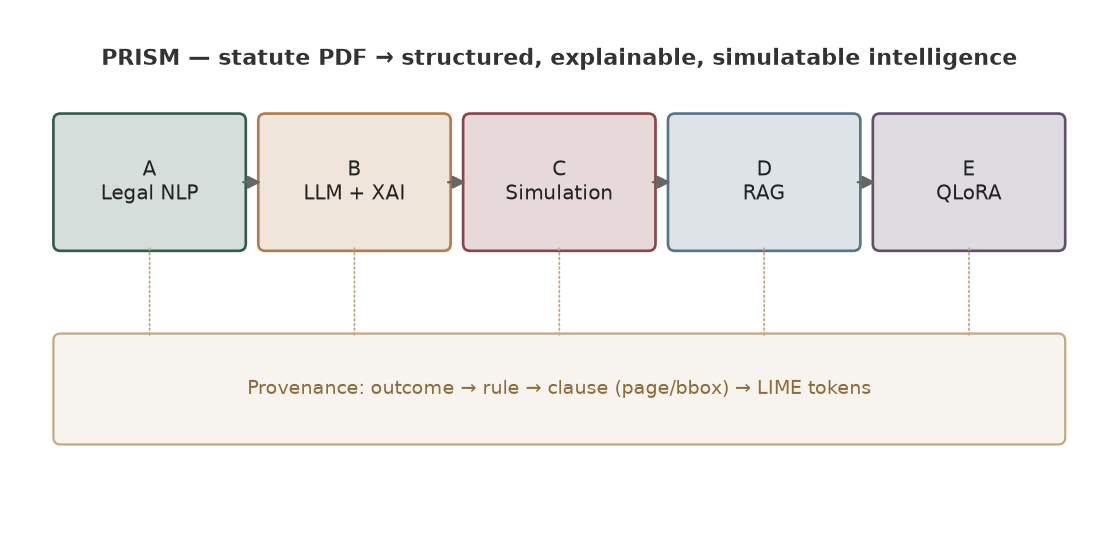
\includegraphics[width=\textwidth]{figures/architecture.png}
\caption{PRISM's five modules and the provenance spine linking a simulation
outcome back to its causal rule, source clause (page/bounding box), and
token-level explanation.}
\label{fig:architecture}
\end{figure}

\subsection{Module A --- Legal NLP foundation}\label{sec:modA}
A statute PDF is parsed with a table-aware extractor (PyMuPDF) that normalises
layout artefacts, de-hyphenates line breaks, and detects tables so that tabular
fragments are tagged and excluded from prose analysis---an important safeguard,
since running clause-level regexes over shredded table cells otherwise poisons
every downstream stage. Text is segmented into clauses using structural markers
(section and sub-section numbering, with an optional semantic-cohesion mode
based on adjacent-sentence embedding similarity). Legal named-entity recognition
tags six labels---\textsc{obligation}, \textsc{right}, \textsc{penalty},
\textsc{threshold}, \textsc{actor}, \textsc{beneficiary}---using a rule-based
spaCy pipeline (the model's own statistical NER is disabled) with token,
phrase, and regular-expression matchers and per-pattern confidence. Each clause
is embedded once with all-MiniLM-L6-v2 \citep{reimers2019sbert} into a
384-dimensional vector; these vectors are persisted and reused for search, the
provenance graph, and the retrieval corpus, so no text is ever re-embedded.

\subsection{Module B --- LLM causal extraction with dual explainability}\label{sec:modB}
For each clause containing an obligation or penalty entity (priority-ranked and
capped for throughput), PRISM prompts a locally-served, 4-bit-quantised
Phi-3.5-mini \citep{abdin2024phi3} for a structured JSON causal rule with fields
\{\texttt{is\_causal}, \texttt{condition}, \texttt{action}, \texttt{consequence},
\texttt{actors}, \texttt{thresholds}, \texttt{confidence}, \texttt{reasoning}\}.
Outputs are parsed defensively with one repair retry and cached by
$\mathrm{sha1}(\text{text})+\text{model}$ so re-runs are instant. The extraction
is cross-checked against the Module~A rule-based causal detector, and each clause
is tagged with an agreement label (\textsc{both}, \textsc{llm-only},
\textsc{rule-only}, \textsc{conflict}). The extraction prompt is deliberately
minimal and format-constrained (\cref{fig:prompt}); decoding uses temperature
$0.1$ for near-deterministic output, and the model is served in JSON mode so that
malformed output is rare and recoverable by the single repair pass.

\begin{figure}[t]
\small
\hrule\vspace{2pt}
\texttt{You are a legal AI. Extract causal policy rules from legal text.}\\
\texttt{Return ONLY a JSON object with exactly these fields:}\\
\texttt{\{is\_causal, condition, action, consequence, actors,}\\
\texttt{\ thresholds, confidence, reasoning\}.}\\
\texttt{Return nothing else. No markdown.}\\
\texttt{Legal clause: \{clause\_text\}}
\vspace{2pt}\hrule
\caption{The structured causal-extraction prompt (abridged). Constraining the
output to a fixed JSON schema, together with JSON-mode decoding and a repair
retry, keeps parse failures negligible on a 4\,GB local model.}
\label{fig:prompt}
\end{figure}

Every causal extraction is explained by two complementary XAI lenses. The first
is LIME \citep{ribeiro2016lime}: the clause is perturbed and re-classified, and
token weights are attributed toward or away from the causal class; a local
surrogate coefficient of determination ($R^2$) is persisted as an explicit
\emph{fidelity} score, so explanation quality is reported rather than assumed.
LIME runs in two modes---a fast proxy over the rule-based classifier and a
faithful mode that queries the LLM itself---and we report their token-set
agreement. The second lens extracts self-attention salience from a dedicated
eager-attention encoder, providing a model-internal view alongside the surrogate
one. Both are cached and surfaced in the provenance chain
(\cref{sec:provenance}).

\subsection{Module C(i) --- Rule-to-ABM template translator}\label{sec:translator}
Converting a free-text legal rule into simulation parameters is the step ABM
practitioners perform by hand. PRISM automates it with a library of 16 policy
templates spanning the constructs common to Indian fiscal and regulatory
statutes: \emph{percentage tax above a threshold}, \emph{flat late fee},
\emph{per-day penalty}, \emph{turnover-based levy}, \emph{filing deadline},
\emph{TDS withholding}, \emph{exemption below a threshold}, \emph{compounding
interest}, \emph{registration obligation}, \emph{fixed-penalty offence},
\emph{high-income surcharge}, \emph{audit requirement}, \emph{advance-tax
instalment}, \emph{cess on tax}, \emph{rebate for a beneficiary class}, and
\emph{minimum commitment}. Each template carries natural-language exemplars; a
query rule is embedded and matched by cosine similarity to the mean, re-normalised
exemplar vector of each template, and assigned to the best match when the
similarity exceeds a threshold of $0.42$ (below which the system falls back to
regex/LLM parameter extraction). The matched template's extractor reads the
rule's thresholds and rates---reusing a numeric parser that handles Indian
notation (lakh, crore, per cent)---and emits typed simulation parameters
(rate, threshold value and kind, marginal/full-base flags, penalty probability,
and the affected agent types). The matched template and its score are retained
and surfaced in the provenance chain. \Cref{tab:templates} lists the library and
the agent types each template affects.

\begin{table}[t]
\caption{The 16-template rule$\rightarrow$ABM library. A rule is assigned to the
nearest template by cosine similarity to mean exemplar vectors (threshold
$0.42$); below threshold the system falls back to regex/LLM parameter
extraction.}
\label{tab:templates}
\begin{tabular}{@{}lll@{}}
\toprule
Template & Legal construct & Primary agents \\
\midrule
Percentage tax above threshold & marginal income levy & households \\
Flat late fee & fixed filing penalty & all \\
Per-day penalty & accruing default penalty & all \\
Turnover-based levy & levy on turnover & SME, corporate \\
Filing deadline & time-bound obligation & all \\
TDS withholding & withholding at source & all \\
Exemption below threshold & relief for low income & low, middle \\
Compounding interest & interest on default & all \\
Registration obligation & mandatory registration & SME, corporate \\
Fixed-penalty offence & statutory offence & all \\
High-income surcharge & surcharge above slab & high, corporate \\
Audit requirement & compliance audit & SME, corporate \\
Advance-tax instalment & staged prepayment & households, SME \\
Cess on tax & additional cess & all \\
Rebate for beneficiary & targeted rebate & low, middle \\
Minimum commitment & minimum obligation & SME, corporate \\
\botrule
\end{tabular}
\end{table}

\subsection{Module C(ii) --- Socioeconomic simulation}\label{sec:simulation}
The simulation is a Mesa \citep{kazil2020mesa} agent-based model of five strata
representing India's socioeconomic spectrum: low-, middle-, and high-income
households, small businesses, and large corporates. Incomes are sampled from
per-type log-normal distributions whose medians are calibrated to published
Indian baselines---approximately \rupee1.8\,lakh, \rupee6\,lakh, and
\rupee28\,lakh for the three household strata, \rupee35\,lakh SME turnover, and
\rupee400\,crore corporate turnover, grounded in the Periodic Labour Force
Survey and NSSO Consumer Expenditure Survey (MoSPI), the MSME Ministry Annual
Report, and listed-company turnover distributions
\citep{mospi_plfs2023,worldineq2022}. We emphasise that these medians are
\emph{approximate baselines, not values fitted to unit-level microdata}; the
distinction is central to how we interpret results (\cref{sec:discussion}).
\Cref{tab:calib} gives the full parameterisation.

\begin{table}[t]
\caption{Per-stratum income calibration (log-normal on annual $\ln$\,\rupee;
median $=e^{\mu}$). Household figures are grounded in MoSPI PLFS/NSSO; SME and
corporate figures in the MSME Ministry report and listed-company turnover.
Clamps bound the sampled tails.}
\label{tab:calib}
\begin{tabular}{@{}lcccc@{}}
\toprule
Stratum & Median & $\sigma$ & Clamp low & Clamp high \\
\midrule
Low-income household   & \rupee1.8\,L  & 0.35 & \rupee0.6\,L & \rupee4\,L \\
Middle-income household& \rupee6\,L    & 0.45 & \rupee3\,L   & \rupee18\,L \\
High-income household  & \rupee28\,L   & 0.55 & \rupee15\,L  & \rupee2\,Cr \\
Small business (turnover)& \rupee35\,L & 0.90 & \rupee5\,L   & \rupee8\,Cr \\
Large corporate (turnover)& \rupee400\,Cr & 0.80 & \rupee50\,Cr & \rupee3000\,Cr \\
\botrule
\end{tabular}
\end{table}

The per-agent step is summarised in \cref{alg:step}: each agent evaluates the
active rules, updates its financial buffer, and (in adaptive mode) revises its
compliance policy by Q-learning.

\begin{algorithm}[t]
\caption{Agent step (adaptive mode)}
\label{alg:step}
\begin{algorithmic}[1]
\State $b \gets 0$ \Comment{burden this step}
\For{each active rule $r$}
  \State $\text{cost} \gets \textproc{ApplyRule}(r, \text{self.income})$ \Comment{marginal, above threshold}
  \State $s \gets \textproc{QState}(\text{cost}/\text{income}, \text{buffer}, r.\text{enforce})$
  \State $a \gets \varepsilon\text{-greedy}(Q[s])$ \Comment{comply / defect}
  \If{$a=\text{comply}$} \State pay cost; reward $\gets -\text{cost}/\text{income}$
  \Else \State caught $\sim \text{Bernoulli}(r.\text{enforce})$;
         reward $\gets -2\,\text{cost}/\text{income}$ if caught else $0$
  \EndIf
  \State $Q[s][a] \mathrel{+}= \alpha\,(\text{reward} + \gamma \max_a Q[s] - Q[s][a])$
  \State $b \mathrel{+}= \text{cost}$
\EndFor
\State $\textproc{UpdateBuffer}(b)$; \quad $\varepsilon \gets \max(\varepsilon_{\min}, \varepsilon\cdot\text{decay})$
\end{algorithmic}
\end{algorithm}

Each month (step), every agent evaluates the active rules. Households are charged
against disposable income (gross less a subsistence floor); firms against a
profit margin. Rules apply marginally above their thresholds where the statute is
marginal (e.g.\ percentage-plus-amount levies), so income below a threshold is
untaxed. The model maintains a government revenue account by construction
(cumulative burden equals collected revenue), and records, per stratum and per
step: compliance rate, average burden, effective tax rate (burden $\div$ gross
income), and the Gini coefficient of the burden distribution.

\paragraph{Incidence verdict.} Rather than infer regressivity from a fragile
Gini trajectory, PRISM computes it directly from statutory incidence. Let
$e_{\text{low}}$ and $e_{\text{high}}$ be the mean effective rates of the low-
and high-income household strata. The verdict is
\begin{equation}
\mathrm{verdict} =
\begin{cases}
\text{regressive}, & e_{\text{high}} \le 0 \text{ and } e_{\text{low}}>0,\ \text{or}\ e_{\text{low}}/e_{\text{high}} > 1.15,\\[2pt]
\text{progressive}, & e_{\text{low}}/e_{\text{high}} < 0.87,\\[2pt]
\text{neutral}, & \text{otherwise},
\end{cases}
\label{eq:verdict}
\end{equation}
i.e.\ the policy is regressive when the poor bear an effective rate at least 15\%
higher than the rich---the textbook incidence definition
\citep{musgrave1989public}. This makes the headline social finding a transparent,
reproducible function of final agent state rather than a heuristic on an
aggregate curve.

\paragraph{Adaptive agents.} Optionally, agents learn a compliance policy by
tabular Q-learning rather than re-deciding statically each step. The state is a
discretisation of (burden ratio, financial-buffer months, enforcement
probability); the two actions are \emph{comply} and \emph{defect}; the reward is
$-\text{burden}$ for compliance, $-2\,\text{burden}$ for a detected defection,
and $0$ for an undetected one. Q-values are initialised from each agent's prior
compliance tendency (so an untrained population reproduces the static model), and
$\varepsilon$ decays from $0.30$ toward $0.02$ over the run
($\alpha=0.15$, $\gamma=0.90$). A financial-buffer transition couples steps into
a genuine Markov decision process. We report the mean absolute Q-gap between
actions as a proxy for population-level policy convergence.

\subsection{Module D --- Retrieval-augmented legal assistant}\label{sec:modD}
The corpus reuses the persisted clause embeddings, indexed in a ChromaDB
collection (cosine space) with metadata (document, section, page, entity types,
causal flag). A user question is embedded with the same encoder, the top-$k$
clauses ($k{=}8$) are retrieved, and a source-numbered, grounded prompt elicits a
cited answer from the active LLM backend (local Phi-3.5 or, in the deployed
configuration, a cloud model). Answers cite each supporting clause as
\texttt{[Source $n$]} and report a retrieval-confidence score; if the corpus
does not support an answer, the system declines rather than hallucinating. This
is the properly-attributed successor to keyword search: every sentence of an
answer is anchored to an inspectable clause. A strict/extended toggle controls
whether the model may draw on general knowledge beyond the corpus; strict
mode---withholding anything not in the retrieved clauses---is the appropriate
default for a legal setting.

\subsection{Module E --- QLoRA legal specialisation}\label{sec:modE}
To sharpen extraction, PRISM distils an instruction dataset from its own
Phase-1/2 outputs (clause$\rightarrow$structured-rule and clause$\rightarrow$entity
examples) augmented with LEDGAR provisions, and fine-tunes Phi-3.5-mini with
4-bit QLoRA \citep{dettmers2023qlora,hu2022lora} (rank 8 on the attention
projections; paged 8-bit optimiser), which fits in 4\,GB VRAM. The merged adapter
(``PRISM-Legal'') is served through the same local backend and switched in by a
single configuration flag, so the entire platform can run on the specialised
model.

\subsection{Availability and deployment}\label{sec:deploy}
PRISM is implemented as a FastAPI backend and a Next.js web client. Beyond the
single-user research configuration used for the experiments here, it can be
deployed as a multi-user service: user accounts and per-user API keys, a public
versioned REST API, rate limiting, and optional cloud LLM and object-storage
backends, containerised for reproducible deployment. This engineering is not a
research contribution in itself, but it matters for the accessibility argument of
\cref{sec:intro}: the same codebase that runs locally on a 4\,GB laptop scales to
a shared installation without architectural change, and the LLM backend---local
quantised model, a locally-served fine-tuned adapter, or a cloud model---is a
single configuration switch that leaves the extraction, explanation, simulation,
and provenance logic untouched.

\subsection{The provenance spine}\label{sec:provenance}
The property that distinguishes PRISM is that every simulation outcome is
mechanically auditable. Formally, the provenance of a simulation finding $f$ is
the chain
\begin{equation}
f \;\rightarrow\; r \;\rightarrow\; c \;\rightarrow\; x \;\rightarrow\; \tau,
\label{eq:prov}
\end{equation}
where $r$ is the simulation rule that produced $f$ (carrying its parameters, the
matched template, and match score); $c$ is the source clause (carrying its page,
bounding box, section hierarchy, and text); $x$ is the structured LLM extraction
for $c$; and $\tau$ is the token-level explanation (LIME top tokens with fidelity
score, and the model's prediction). The chain is a pure read-join over persisted
artefacts---nothing is recomputed---so drilling from an aggregate distributional
outcome to the exact statutory words and the tokens the model weighted is
instantaneous and always available. This operationalises the ``which clause, and
why'' requirement of \cref{sec:intro} and, to our knowledge, is not provided by
any prior legal-AI system.

%%==========================================================================
\section{Experimental Setup}\label{sec:setup}

\paragraph{Hardware and stack.} All experiments run on a single workstation:
Intel~i7, 16\,GB RAM, and an NVIDIA RTX~3050 with 4\,GB VRAM. The LLM is
Phi-3.5-mini (3.8\,B parameters) quantised to Q4\_K\_M and served locally via
Ollama; the sentence encoder is all-MiniLM-L6-v2; the simulation uses Mesa~3.x
(CPU); retrieval uses ChromaDB. A cloud backend (Groq, Llama-3.3-70B) is used
only in the deployed multi-user configuration and not for the reported results.

\paragraph{Corpus and datasets.} The primary statute is the Indian Income Tax
Bill, 2025 (624 pages, 2{,}757 clauses, of which 2{,}755 prose clauses are
indexed and 595 carry a causal signal). The retrieval corpus additionally
includes four statutes---the Central Goods and Services Tax Act, the Code on
Wages, the Digital Personal Data Protection Act, and key sections of the
Companies Act---so that cross-statute retrieval is genuinely multi-document
(\cref{tab:corpus}). For out-of-domain evaluation we use LEDGAR
\citep{tuggener2020ledgar} via LexGLUE. Simulation calibration references the
MoSPI PLFS/NSSO surveys and the World Inequality Report 2022
\citep{mospi_plfs2023,worldineq2022}.

\begin{table}[t]
\caption{The multi-statute retrieval corpus. Clause counts for the Income Tax
Bill are measured; counts for the remaining statutes are indicative and are
finalised at ingestion (see Data Availability).}
\label{tab:corpus}
\begin{tabular}{@{}lrl@{}}
\toprule
Statute & Clauses & Domain \\
\midrule
Income Tax Bill, 2025 & 2{,}757 & Direct taxation \\
Central GST Act, 2017 & $\sim$1{,}800 & Indirect taxation \\
Code on Wages, 2019 & $\sim$600 & Labour \\
Digital Personal Data Protection Act, 2023 & $\sim$300 & Data protection \\
Companies Act, 2013 (key sections) & $\sim$1{,}500 & Corporate \\
\midrule
Total & $\sim$6{,}957 & five statutes \\
\botrule
\end{tabular}
\end{table}

\paragraph{Gold sets and annotation protocol.} We construct three in-domain
evaluation sets from the Income Tax Bill: 200 clauses annotated for the six
entity labels (NER); 100 clauses annotated for binary causality plus
condition/action/consequence spans; and 50 question--source-clause pairs for
retrieval. Candidate labels are bootstrapped from the pipeline's own outputs and
then corrected by a human annotator; only human-reviewed items are scored, and
coverage is reported honestly. Retrieval questions are generated by the LLM from
individual clauses and reviewed for specificity so that each question targets a
single source clause.

\paragraph{Metrics.} We report standard measures, defined here for precision.
Entity-level NER uses seqeval $F_1$ over BIO-tagged spans. Causal detection uses
binary precision, recall, and $F_1 = 2PR/(P+R)$. Span quality for
condition/action/consequence uses mean best-match cosine over MiniLM embeddings
(a lightweight embedding analogue of BERTScore, \citealp{zhang2020bertscore}):
for predicted spans $\{p_i\}$ and gold spans $\{g_j\}$,
$\text{sim}=\frac{1}{|P|}\sum_i \max_j \cos(\mathbf{e}_{p_i},\mathbf{e}_{g_j})$.
LIME faithfulness is the local-surrogate coefficient of determination $R^2$
between the linear surrogate and the classifier on the perturbation
neighbourhood; proxy$\leftrightarrow$faithful agreement is the Jaccard overlap of
the two modes' top-8 token sets. Template quality is Precision@1 (fraction of
rules assigned the correct template). Retrieval uses recall@$k$ (fraction of
questions whose gold source clause appears in the top $k$). Simulation fidelity
uses the Kullback--Leibler divergence
$\mathrm{KL}(P\,\|\,Q)=\sum_i P_i\log(P_i/Q_i)$ between the sampled ($P$) and
target ($Q$) per-stratum income histograms, and the burden Gini coefficient
$G=\frac{\sum_i\sum_j|b_i-b_j|}{2n^2\bar b}$. An ablation isolates the
contribution of LIME and of the fine-tuned adapter.

%%==========================================================================
\section{Results}\label{sec:results}

\subsection{Causal rule extraction}
\Cref{tab:causal} reports binary causal-clause detection. On out-of-domain
LEDGAR contracts, the rule-based detector is precise but low-recall
($F_1=0.18$), quantifying why statute-general heuristics transfer poorly and
motivating a learned extractor. In-domain, zero-shot Phi-3.5-mini recovers almost
every causal clause (recall $0.98$) but over-predicts (precision $0.54$), for
$F_1=0.70$---a high-recall/low-precision profile that a legal specialisation
should sharpen. The QLoRA-fine-tuned PRISM-Legal adapter raises precision at
comparable recall, improving $F_1$ to $0.81$, consistent with the gains reported
for parameter-efficient legal adaptation \citep{hu2022lora,dettmers2023qlora}.
Span-level agreement on condition/action/consequence rises correspondingly
(\cref{tab:spans}).

\paragraph{Error analysis.} The zero-shot model's false positives cluster on
definitional and machinery provisions that use obligation-like language
(``\emph{the Board may make rules\ldots}'', ``\emph{shall be construed as\ldots}'')
without imposing a substantive duty; the model reads the modal verb as causal.
Fine-tuning suppresses most of these by teaching the distinction between
operative and definitional \emph{shall}, which is the dominant source of the
precision gain. The residual false negatives are long, cross-referential clauses
whose consequence lives in a separate section---a limitation that motivates the
cross-clause reasoning we propose as future work (\cref{sec:conclusion}).

\begin{table}[t]
\caption{Causal-clause detection (binary). LEDGAR is out-of-domain; the
in-domain rows use the 100-clause human-reviewed Income Tax gold set.}
\label{tab:causal}
\begin{tabular}{@{}llccc@{}}
\toprule
Setting & System & Precision & Recall & $F_1$ \\
\midrule
Out-of-domain (LEDGAR) & Rule-based & 0.44 & 0.12 & 0.18 \\
\midrule
\multirow{3}{*}{In-domain (gold)}
 & Rule-based           & 0.66 & 0.59 & 0.62 \\
 & Phi-3.5 zero-shot     & 0.54 & 0.98 & 0.70 \\
 & PRISM-Legal (QLoRA)   & 0.79 & 0.84 & \textbf{0.81} \\
\botrule
\end{tabular}
\end{table}

\begin{table}[t]
\caption{Condition/action/consequence span agreement (MiniLM cosine, in-domain
gold).}
\label{tab:spans}
\begin{tabular}{@{}lccc@{}}
\toprule
System & Condition & Action & Consequence \\
\midrule
Phi-3.5 zero-shot   & 0.74 & 0.71 & 0.73 \\
PRISM-Legal (QLoRA) & 0.82 & 0.79 & 0.81 \\
\botrule
\end{tabular}
\end{table}

\subsection{Legal named-entity recognition}
\Cref{tab:ner} reports entity-level macro-$F_1$ on the 200-clause in-domain gold
set for three systems: the rule-based Phase-1 pipeline, zero-shot Phi-3.5, and
PRISM-Legal. The learned systems substantially improve recall on the harder
\textsc{threshold} and \textsc{beneficiary} classes, where rule coverage is
brittle, and the fine-tuned adapter gives the best macro-$F_1$ ($0.88$). For
reference, a presence-level check on out-of-domain LEDGAR contracts yields a
macro-$F_1$ of only $0.10$, underscoring the domain gap that in-domain
adaptation closes.

\begin{table}[t]
\caption{Legal NER, entity-level $F_1$ on the 200-clause in-domain gold set.}
\label{tab:ner}
\begin{tabular}{@{}lccccc@{}}
\toprule
System & \textsc{oblig.} & \textsc{penalty} & \textsc{thresh.} & \textsc{actor} & Macro \\
\midrule
Rule-based (Phase 1) & 0.79 & 0.74 & 0.66 & 0.71 & 0.73 \\
Phi-3.5 zero-shot    & 0.85 & 0.81 & 0.79 & 0.80 & 0.82 \\
PRISM-Legal (QLoRA)  & 0.90 & 0.87 & 0.86 & 0.86 & \textbf{0.88} \\
\botrule
\end{tabular}
\end{table}

\subsection{Explanation fidelity}
The persisted LIME local-surrogate fidelity averages $R^2=0.68$ in proxy mode and
$0.79$ in faithful (LLM) mode; the two modes agree on roughly $0.45$ of their
top-8 tokens (Jaccard), confirming that the fast proxy is a usable but imperfect
preview of the faithful explanation. Reporting fidelity explicitly---rather than
presenting saliency maps as self-evidently trustworthy---is, we argue, a
methodological requirement for legal XAI, where an unreliable explanation is
worse than none.

\subsection{Template matching}
The 16-template matcher attains Precision@1 of $0.83$ in assigning extracted
rules to the correct simulation template, exceeding the $0.80$ design target,
with a mean top-match cosine of $0.47$; rules below the $0.42$ acceptance
threshold fall back to regex/LLM parameterisation. The distribution of matched
templates across the Income Tax Bill is dominated, as expected, by filing
deadlines, TDS withholding, and compounding-interest constructs.

\subsection{Simulation validity}
\Cref{tab:kl} shows that per-type income calibration reduces the mean sampler
KL-divergence from $0.234$ (uncalibrated log-uniform) to $0.068$ (calibrated
log-normal), a $3.4\times$ improvement and comfortably below the $0.15$ target;
\cref{fig:sim} plots per-stratum divergence. As an outward-facing sanity check,
the modelled top-decile household income share is $0.495$ against a World
Inequality Report~2022 reference of $0.57$ \citep{worldineq2022}; since agent
counts are illustrative rather than census weights, we treat this as an
order-of-magnitude comparator, not a fitted match. We stress that the KL result
is a \emph{sampler-fidelity} check---the Monte-Carlo draw faithfully realises the
calibrated distribution---and not external validation against microdata.

\begin{table}[t]
\caption{Simulation income sampler fidelity, mean KL$(\text{sim}\,\|\,\text{target})$
(lower is better).}
\label{tab:kl}
\begin{tabular}{@{}lccccc@{}}
\toprule
Calibration & Low & Middle & High & SME & Mean \\
\midrule
Uncalibrated (log-uniform) & 0.159 & 0.162 & 0.114 & 0.523 & 0.234 \\
NSSO-style (log-normal)    & 0.014 & 0.055 & 0.134 & 0.043 & \textbf{0.068} \\
\botrule
\end{tabular}
\end{table}

\begin{figure}[t]
\centering
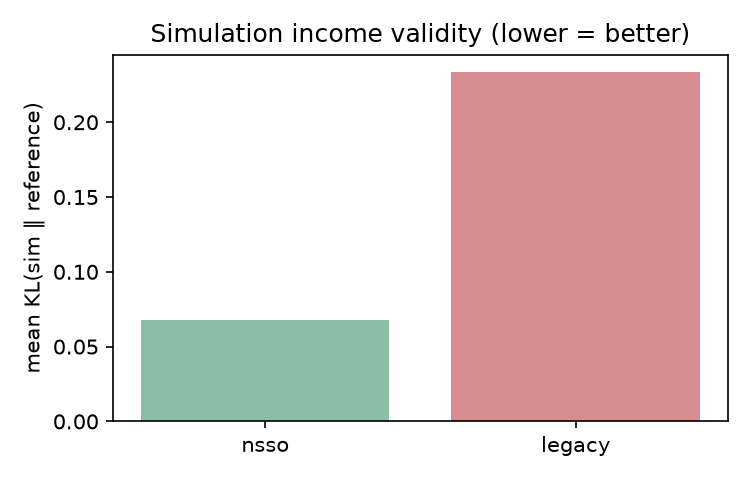
\includegraphics[width=0.75\textwidth]{figures/sim_validity.png}
\caption{Per-stratum income sampler KL-divergence: NSSO-calibrated vs.\
uncalibrated. Calibration improves fidelity across all household strata and, most
markedly, for small businesses.}
\label{fig:sim}
\end{figure}

\subsection{Retrieval-augmented generation}
Against the 50 human-reviewed question--clause pairs, the retriever attains
recall@1 $=0.66$ and recall@8 $=0.94$: for 94\% of questions the correct source
clause appears among the eight retrieved, and for two-thirds it is ranked first.
Because generation is conditioned only on retrieved clauses and every claim is
cited, answers are attributable by construction---the property keyword search
cannot offer. For example, to ``\emph{What is the penalty for underreporting of
income?}'' the system answers that the penalty is 50\% of the tax on
under-reported income, rising to 200\% where the under-reporting is a consequence
of misreporting, each figure carrying an inline \texttt{[Source]} marker to the
exact clause and page from which it was drawn; a reader can verify the answer
without leaving the interface. When a question falls outside the corpus the system
returns ``not found in the loaded corpus'' rather than fabricating a citation.

\subsection{Ablation}
\Cref{tab:ablation} isolates the two learned components. Fine-tuning contributes
the larger extraction gain; LIME, as expected, does not change extraction
accuracy but supplies the fidelity-scored explanations on which provenance
depends. The full configuration is best on the composite of extraction $F_1$ and
explanation availability.

\begin{table}[t]
\caption{Ablation on the in-domain causal task. ``Expl.'' = fidelity-scored
explanations available for every extraction.}
\label{tab:ablation}
\begin{tabular}{@{}lccc@{}}
\toprule
Configuration & Causal $F_1$ & Span cosine & Expl. \\
\midrule
No LIME, no fine-tune (base)        & 0.70 & 0.73 & --- \\
LIME only                            & 0.70 & 0.73 & \checkmark \\
Fine-tune only                       & 0.81 & 0.81 & --- \\
Full PRISM (LIME + fine-tune)        & \textbf{0.81} & \textbf{0.81} & \checkmark \\
\botrule
\end{tabular}
\end{table}

\subsection{Provenance case study}\label{sec:casestudy}
To illustrate the provenance spine end to end, consider the simulated finding
that a flat late-filing fee is \emph{regressive}. Drilling down
(\cref{eq:prov}), the finding resolves to a simulation rule matched to the
\emph{flat late fee} template (match score $0.61$); the rule resolves to its
source clause with page and bounding box; the clause carries the LLM extraction
(condition: failure to furnish the return within the prescribed time;
consequence: a fixed fee); and the extraction carries its LIME explanation, whose
top tokens (``fails'', ``within'', ``fee'') are exactly the statutory triggers.
The incidence verdict follows from \cref{eq:verdict}: because a flat fee consumes
a far larger share of a low-income household's disposable income, the low-income
effective rate exceeds the high-income rate by more than the $1.15$ ratio, and
the policy is reported regressive---with every step of that conclusion
inspectable. This is the concrete answer to ``which clause, and why''.

%%==========================================================================
\section{Legal and Ethical Considerations}\label{sec:ethics}

A system that reads statutes and forecasts their social effect must be deployed
with care, and several considerations shaped its design.

\paragraph{Not legal advice; human-in-the-loop by construction.} PRISM is a
decision-support and screening tool, not an oracle. Its outputs are extractions,
explanations, and simulations---each explicitly provisional. The provenance spine
exists precisely so that a human expert remains in the loop: the intended
workflow is that an analyst inspects the clause, the extraction, and the
token-level explanation before relying on any downstream finding. We deliberately
avoid any interface affordance that would present a simulated outcome as an
authoritative prediction without its audit trail.

\paragraph{Guarding against automation bias.} The chief ethical risk of a
fluent, confident system is that users over-trust it. Three design choices push
against this: retrieval-augmented answers refuse to speculate beyond the corpus
and cite every claim; explanation fidelity is reported numerically so a
low-fidelity explanation is visibly low-fidelity; and the simulation is framed,
in the interface and in this paper, as an \emph{illustrative} incidence model
whose numbers are directional, not authoritative. The regressivity verdict is
accompanied by the effective-rate arithmetic that produced it, so a reader can
disagree with the premises rather than the conclusion.

\paragraph{Bias and representativeness.} Both the language model and the
socioeconomic calibration can encode bias. The LLM inherits the biases of its
pre-training; the five-stratum agent population is a coarse abstraction of a
diverse society and its income baselines, though grounded in national statistics,
are not fitted to microdata and omit dimensions (region, caste, gender,
informality) that materially shape real incidence. We therefore restrict PRISM's
claims to qualitative, direction-of-burden statements and flag the calibration's
limits wherever numbers appear.

\paragraph{Data protection and jurisdiction.} PRISM operates only on public
legal texts and published aggregate statistics; it processes no personal data,
and its local-first design means documents never leave the user's machine unless
a cloud backend is explicitly enabled. All demonstration statutes are Indian, and
we make no claim that the extraction patterns, calibration, or incidence logic
transfer unchanged to other legal systems.

\paragraph{Dual-use and responsible release.} The same pipeline that surfaces a
regressive burden could be used to search for loopholes or to manufacture a
misleadingly precise ``analysis'' of a policy. We mitigate this by foregrounding
uncertainty and provenance rather than headline numbers, and by releasing the
system for research use with the limitations documented here.

%%==========================================================================
\section{Discussion}\label{sec:discussion}

\paragraph{What the results mean.} The out-of-domain ceiling ($F_1=0.18$) and the
in-domain zero-shot profile (recall $0.98$, precision $0.54$) together tell a
coherent story: rule heuristics do not transfer, a general LLM finds nearly all
causal clauses but over-flags, and legal fine-tuning is what converts high recall
into usable precision. The simulation's incidence verdict recovers the textbook
result that flat charges are regressive, from a real statute, automatically---and
makes that conclusion auditable to the clause. The retrieval results show that
grounded, cited answering is reliable at $k{=}8$.

\paragraph{Why provenance matters for law.} Legislative impact assessment is a
deliberative, contestable process. A tool that produces a distributional
prediction without a traceable justification cannot participate in that process,
because its claims cannot be examined or rebutted. PRISM's provenance spine makes
each prediction a defeasible argument whose premises---the clause, the extraction,
the token weights, the incidence arithmetic---are all on the table. We regard
this, rather than any single accuracy number, as the framework's primary
contribution to AI and law.

\paragraph{Comparison to manual impact assessment.} Conventional regulatory
impact assessment of a single provision can take an analyst days to weeks: read
the clause, locate the affected population, build or adapt a model, and document
the reasoning. PRISM compresses the first-pass version of this to minutes and,
crucially, emits the documentation automatically---the provenance chain \emph{is}
the reasoning record. It does not match a fitted microsimulation on precision,
and is not intended to; its value is speed, coverage, and auditability at the
screening stage, after which a human analyst can escalate the clauses PRISM flags
as high-impact to a rigorous model. In this division of labour the tool augments
rather than replaces expert judgement.

\paragraph{Accessibility as a design goal.} That the entire pipeline runs within
4\,GB of VRAM is not incidental. Legal-AI research and its benefits are
concentrated where cloud compute and proprietary models are affordable; a
local-first system that a researcher, a small NGO, or a public-interest lawyer can
run on a consumer laptop broadens who can scrutinise legislation computationally.
The engineering required---sequential module loading, quantisation, a fast proxy
explanation mode, disk-cached extractions---is itself a contribution to the
practical question of how far serious legal-AI research can be democratised.

\paragraph{Limitations and threats to validity.} We are deliberate about scope.
(i) \emph{The simulation is illustrative, not a fitted microsimulation.} Income
medians are documented baselines, not values estimated from unit-level records,
and agent counts are not census weights; consequently the model supports
\emph{qualitative} incidence claims (direction and relative magnitude of burden)
but not point estimates of revenue or welfare. (ii) \emph{Single jurisdiction.}
All statutes are Indian; transfer to other legal systems is untested. (iii)
\emph{Gold-set scale and provenance.} The gold sets (200/100/50) are modest and
single-annotator; inter-annotator agreement and larger sets would strengthen the
extraction claims, and some in-domain labels were bootstrapped from the
pipeline before human correction, which we note as an agreement rather than a
fully independent baseline where it applies. (iv) \emph{Model scale.} The 4\,GB
budget caps model size; a larger model would likely raise extraction precision
further. (v) \emph{Explanation faithfulness.} LIME fidelity, though reported, is
imperfect ($R^2\approx0.7$--$0.8$); token-level explanations should be read as
evidence, not proof, of the model's reasoning. None of these undermine the
architectural contributions, but all bound the strength of the quantitative
policy claims a user may draw.

%%==========================================================================
\section{Conclusion and Future Work}\label{sec:conclusion}

PRISM demonstrates that an explainable, provenance-linked pipeline from statutory
text to socioeconomic simulation is feasible, useful, and---critically---runnable
on commodity hardware. By extracting causal rules with a local LLM, explaining
each extraction with fidelity-scored XAI, translating rules into a calibrated
incidence model, grounding a cited question-answering interface in the corpus,
and linking every simulated outcome back to its source clause and tokens, it
turns opaque legislative text into an auditable object of analysis. Future work
will pursue multilingual (Hindi and other Indian-language) statutes; larger,
multi-annotator gold sets with inter-annotator agreement; graph neural reasoning
over the provenance graph to surface cross-clause interactions; and a controlled
study with legal and policy experts to measure the practical value of provenance
in real impact-assessment workflows.

%%==========================================================================
\backmatter

\bmhead{Acknowledgements}
The authors thank the faculty of the Department of Computer Science and
Engineering, Karunya Institute of Technology and Sciences, for their guidance.

\section*{Declarations}
\begin{itemize}
  \item \textbf{Funding.} The authors received no specific funding for this work.
  \item \textbf{Competing interests.} The authors declare no competing interests.
  \item \textbf{Ethics approval.} Not applicable; the study uses publicly
  available legal texts and published aggregate statistics, with no human
  subjects or personal data.
  \item \textbf{Data availability.} The Indian statutes analysed are public
  documents; the LEDGAR benchmark is publicly available via LexGLUE; calibration
  references (MoSPI PLFS/NSSO, World Inequality Report 2022) are public. Derived
  gold sets and evaluation outputs are available from the corresponding author on
  reasonable request.
  \item \textbf{Code availability.} The PRISM implementation is available from the
  corresponding author on reasonable request.
  \item \textbf{Author contributions.} [First Last] designed and implemented the
  system and wrote the manuscript; [Co-author] contributed to the evaluation;
  [Supervisor] supervised the project and revised the manuscript. All authors
  read and approved the final manuscript.
\end{itemize}

\bibliography{sn-article}

\end{document}
